
\resetcounters

\markboth{Teuben et al.}{Science Mining and Characterization of ALMA Large Data Cubes}

\title{Science Mining and Characterization of ALMA Large Data Cubes}
\author{Peter~Teuben,$^1$ Cheuk~Yiu~Ip,$^2$ Lee~Mundy,$^1$ and Amitabh~Varshney$^2$
\affil{$^1$Astronomy Department, University of Maryland, College Park}
\affil{$^2$Institute for Advanced Computer Studies, University of Maryland, College Park}}

\aindex{Teuben, P.}
\aindex{Ip, C. Y.}
\aindex{Mundy, L.}
\aindex{Varshney, A.}

%% start cut and paste body 
\begin{abstract}

We are using Multilevel Segmentation of the Intensity-Gradient
Histograms and Description Vectors to show unique ways to visualize
and analyse complex structures in large ALMA data cubes. In particular
higher dimensional data cubes with many spectral lines are a challenge
both algorithmically and visually. In this poster we show some examples
of both theoretical and observational data cubes and how novel
techniques developed outside of our field can be applied to Astronomy,
and compare them to more traditional methods used in Astronomy,
such as ClumpFind.

\end{abstract}

\section{Introduction}

Large 4-dimensional datacubes that telescopes such as ALMA are now producing,
provide an extra challenge for visualization and analysis. For each voxel in
the traditional RA-DEC-VEL datacube we now have information on a large number
of molecular transitions. Or one could use a single long 3D cube, or a series
of 3D cubes, one for each molecular transition.
Apart from automatically detecting the emission
and categorizing their properties, correllations between the different species
can lead to a deeper understanding of the underlying phyics and chemistry
in the emission regions.

We will introduce a new method to find and categorize emission, and
compare this to a more traditional method of assigning clumps to the
emission structure.

\section{ALMA data}

We obtained some ALMA data for NGC 253, organized in a single 350 x 350 x 1500
cube, but where the 3rd (spectral) 
axis are really 15 different windows (and not all equal in
size) representing 15 different molecular transitions.


\section{Saliency Maps}

This procedure effectively reduces millions of pixels to hundreds or
tens of parameterized objects.  We present an automatic algorithm that
identify salient regions from a radio astronomy image and we
parameterized and index these regions by fitting ellipses to the
identified regions.  Our algorithm is inspired by the computational
saliency model which detects regions of interest from images.

% {\it this still needs (optionally) to be extended to 3D in our case of
% velocity datacubes}

A saliency map shows which part of an image is likely to attract the
most attention of the low-level human visual system.
\cite{itti98:_model_of_salien_based_visual} have proposed a
computational model of visual saliency by using multiscale image
processing.  Multiscale image processing techniques analyze an image
at different scales to simulate the retinal receptive fields.  Their
image saliency model aggregates the results from three features of an
image -- intensity, color opponencies, and orientation. For this
astronomy application we only consider the signal intensity for the
computing image saliency. See also \citep{ip2012hierarchical}.
% describe this a bit more?

The traditional algorithm for computing a saliency map of an image is essentially
the following:

%\begin{align}
\begin{eqnarray*}
  \label{eqn:sal}
  F      & \leftarrow & \mathrm{Image}, \\
  G_{j}   & =          & \mathcal{G}(j) \otimes F, \quad j \in{\sigma,2\sigma,4\sigma,8\sigma,16\sigma
 \cdots}\\
  D_{j,k}  & =         & |G_{i,j} - G_{i,k}|, \quad k \in \{4j,8j\}\\
\end{eqnarray*}
%\end{align}


We convolve the images $F$
with Gaussian kernels, $\mathcal{G}$, at different scales $j$.  We
then find contrasting regions by computing the difference of Gaussians
($DoG$) images at each scale, $G_{j}$.  We compute the $DoG$ images
at scales $\{\sigma,4\sigma\}, \{\sigma,8\sigma\}$.  The $DoG$
operation mimics the contrast detecting receptive fields of retinal
ganglion cells.  Fig 1. shows the $DoG$ operation
extracts contrasting cars from the background.  Normally a
normalization procedure is applied to extract the most salient feature
from the image.  However, as we are interested in peak regions, in
addition to the dominating peak, we skipped this peak promotion
normalization.  We also analyze these $DoG$ map separately.

We threshold the $DoG$ images to extract the salient pixels and we
group these salient pixels into segments.  We first suppress pixels
with low signal by thresholding.  Then, we segment these $DoG$ images
by finding the connected components with the region growing method.
We perform this thresholding and pixel grouping operation at all
scales of the image.

For each segment, we fit ellipses to the pixels by using principal
component analysis.  The center of the ellipse is given by the center
of mass of the pixels.  The angle, major, and minor axes can be
computed by decomposing the covariance matrix of the pixels locations.
We can use these parameters along with saliency measures at different
scales to index each of these segments.

\begin{figure}[ht!]
\centering
% \includegraphics[scale=0.5]{s3-ell-0.eps}
\includegraphics[scale=0.5]{part9/Teuben_P059/s3-ell-0.eps}
\caption{Clumps identified from saliency maps}
\label{fig:teuben1}
\end{figure}

% probably should be using a long cut example, not the squarish cut 
% 

\section{Comparing}

In order to compare the two methods, we used NEMO \citep{nemo} to
construct a known model rotating galactic
disk with a set number of Giant Molecular Clouds (GMC's): N=100, 1000, and 10000,
and constructed synthetic RA-DEC-VEL datacubes.
The last one in particular is showing serious blending. The synthetic datacubes
were analyzed with the ClumpFind \citep{clumpfind} program, as implemented
in the MIRIAD \citep{miriad} package.
\ooindex{Clumpfind, ascl:1107.014} 
\ooindex{MIRIAD, ascl:1106.007}
\ooindex{NEMO, ascl:1010.051}

On its most basic level, the experiments with 100, 1000 and 10,000 clumps returned
70, 248 and 255 clumps resp. in ClumpFind, whereas our new method resulted in
67, 338 and 568 clumps resp. Results are summarized in Table 1.  

% we don't have any total mass assignments for the saliency method yet. could live without

\begin{table}[!ht]
\caption{Recovery of Number and total Mass of
clumps in a rotating galactic disk   (1=clumpfind  2=saliency maps)}
\smallskip
\begin{center}
{\small
\begin{tabular}{lccccc}
\tableline
\noalign{\smallskip}
N    &  NC1   & NC2   & M1   & dM1 & M2  \\     
\noalign{\smallskip}
\tableline
\noalign{\smallskip}
  100  &  70   &  67   & 0.85 & 0.03 & ?  \\
 1000  & 248   & 338   & 0.44 & 0.05 & ?  \\
10000  & 255   & 568   & 0.57 & 0.09 & ?  \\

\noalign{\smallskip}
\tableline
\end{tabular}
}
\end{center}
\end{table}





\begin{figure}[ht!]
\centering
% \includegraphics[scale=0.5]{gmc1.eps}
\includegraphics[scale=0.45]{part9/Teuben_P059/gmc1.eps}
\caption{Simulation of N=100 (left) and N=1000 (right) GMC's in a galactic disk.}
\label{fig:teuben2}
\end{figure}



\acknowledgements We thank Alberto Bolatto and Steve Warren for sharing their 
NGC 253 data before publication.



%% end cut and paste body 


\bibliographystyle{asp2010}
\bibliography{editor}
